\newpage
\section*{Referencias}
\textbf{Básico: }
\begin{itemize}
	\item \textit{Problema 1.} Creado.
	\item \textit{Problema 2.} \textbf{Creado }.
	\item \textit{Problema 3.} OBMEP 2010, Nivel 1, problema 32.
	\item \textit{Problema 4.} Creado.
	\item \textit{Problema 5.} Problema 6, taller de Áreas de la Universidad de Antioquia.
\end{itemize}

\textbf{Avanzado: }
\begin{itemize}
	\item \textit{Problema 1.} Problema 3 Geometría Nivel 2 Aula 4 , Programa Olimpico Treinamento POTI.
	\item	\textit{Problema 2.} Problem 8, Section ''Integers`` (p. 3) del libro ''Mathematical problems and puzzles`` de S. Straszeuiez. 
	\item	\textit{Problema 3.} Creado.
	\item	\textit{Problema 4.} Problema 10, taller de Polinomios de la Universidad de Antioquia.
	\item	\textit{Problema 5.} Creado.
\end{itemize}

%------------------------------------------------------------------------------------------------------------   
%----------------------------------                        BASICO                       ---------------------------------- 
%------------------------------------------------------------------------------------------------------------ 

\newpage
\section{Nivel Básico}\label{basico:2020_10_octubre}

\begin{center}
	\fbox{\fbox{\parbox{6in}{\centering
				\textbf{Tiempo mínimo: } 2 horas y 30 minutos.\\
				\textbf{Tiempo máximo: } 4 horas.\\	
				\textbf{Procedimientos: }Cada problema debe estar resuelto por escrito, en forma detallada, todos los pasos seguidos para su resolución deben estar bien explicados. Se le brindarán unas hojas grapadas, en la \textit{parte de enfrente} de cada hoja debe estar la solución de los problemas, la \textit{parte posterior} no se leerá pero las operaciones y cálculos deben hacerlos allí. \\
				\textbf{Puntaje: }Cada problema vale 50 puntos, son 5, para un total de 250 puntos.
				}}}
\end{center}

\begin{enumerate}
	\item \textbf{(50 puntos)}.  Cuántos triángulos isósceles diferentes de perímetro 30cm se pueden construir con lados de longitud entera? 
			
	\item \textbf{(50 puntos)}. Un mago le pide a un niño que piense tres números naturales diferentes. El mago es un gran mago y siempre logra adivinar los números que las personas están pensando, pero esta vez se le ha quedado su sombrero en casa y ha perdido toda la magia. Para intentar adivinar los números que el niño está pensando, le pide que le diga cuánto es el producto de ellos, a lo que el niño le responde: 'El producto de los numeros que estoy pensando es  210'. El mago sigue sin adivinar, y el niño le dice otra pista: 'Ninguno de mis números es el 1'. Ayudale al mago diciendole todos los posibles números que puede estar pensando el niño.
			
	
	\item \textbf{(50 puntos)}. Una correa cuadriculada tiene 5 cuadraditos de altura y 250 cuadraditos de ancha como se muestra en la figura \ref{fig:correa_cuadraditos}. Algunos cuadraditos están pintados de gris en sig-sag, comenzando en la izquierda y continuando hacia la derecha con el mismo patrón hasta terminar la correa. Cuántos cuadraditos no están pintados?
				
	\begin{figure}[H]
		\centering
		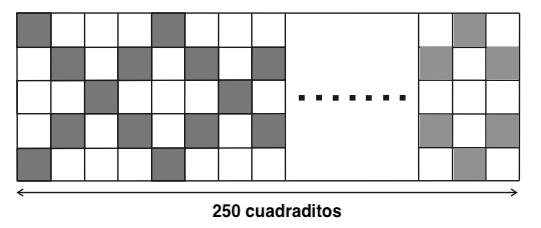
\includegraphics[width=0.8\linewidth]{2020_10_10/imgs/basico_faja_cuadraditos}
		\caption{Correa de cuadraditos.}
		\label{fig:correa_cuadraditos}
	\end{figure}

	\item \textbf{(50 puntos)}. Juan y Sofía están organizando la biblioteca del colegio. La biblioteca solamente tiene 12 libros, todos diferentes. Juan y Sofía los quieren organizar y se dan cuenta que hay 5 en español, 3 en inglés y 4 en francés. Si para organizarlos deciden colocarlos todos sobre un mismo estante,
	\begin{enumerate}[label=\Alph*)]
		\item de cuántas maneras diferentes pueden organizar los libros?
		\item de cuántas maneras diferentes pueden organizar los libros, si los libros que están escritos en el mismo idioma deben quedar juntos?
	\end{enumerate}
		
	\item \textbf{(50 puntos)}. En la figura \ref{fig:area_faja_cuadrado}, el cuadrado $ABCD$ tiene lado de longitud $2cm$. $M$ es punto medio de $BC$ y $N$ es punto medio de $DC$. Calcular el área del cuadrilátero $DNMB$?
	
	\begin{figure}[H]
		\centering
		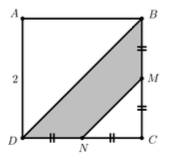
\includegraphics[width=0.5\linewidth]{2020_10_10/imgs/area_faja_cuadrado}
		\caption{Cuadrado $ABCD$ de lado $2cm$. }
		\label{fig:area_faja_cuadrado}
	\end{figure}
	
\end{enumerate}



%------------------------------------------------------------------------------------------------------------   
%----------------------------------                        AVANZADO                       ---------------------------------- 
%------------------------------------------------------------------------------------------------------------ 

\newpage
\section{Nivel Avanzado}\label{avanzado:2020_10_octubre}

\begin{center}
	\fbox{\fbox{\parbox{6in}{\centering
				\textbf{Tiempo mínimo: } 2 horas y 30 minutos.\\
				\textbf{Tiempo máximo: } 4 horas.\\		
				\textbf{Procedimientos: }Cada problema debe estar resuelto por escrito, en forma detallada, todos los pasos seguidos para su resolución deben estar bien explicados. Se le brindarán unas hojas grapadas, en la \textit{parte de enfrente} de cada hoja debe estar la solución de los problemas, la \textit{parte posterior} no se leerá pero las operaciones y cálculos deben hacerlos allí. \\
				\textbf{Puntaje: }Cada problema vale 50 puntos, son 5, para un total de 250 puntos.
	}}}
\end{center}


\begin{enumerate}
	\item \textbf{(50 puntos)}. Sea $ABC$ un triángulo equilatero de lado $20cm$. Una recta pasa por el punto medio $M$ en el lado $AB$ y un punto $N$ en el lado $AC$ y corta a la recta $\overleftrightarrow{BC}$ en el punto $P$ de modo que $CP=12cm$. Hallar la longitud de $NA$.
	

	\item \textbf{(50 puntos)}. Probar que el número $2^{55}+1$ es divisible por 11.
	

	\item \textbf{(50 puntos)}.  Cuántas palabras diferentes se pueden crear con usando exactamente las mismas letras de la palabra \[\textit{''MARAVILLA``}?\] (\textbf{Nota}: ''MARAVILLA`` tiene nueve letras. Una palabra es la union deletras, por ejemplo: ''MARALLAVI``. ).

	\item \textbf{(50 puntos)}. Sean $r_1$ y $r_2$ las raices (soluciones) de la ecuación cuadrática $x^2+px+q=0$. Si se sabe que $r_1 - 2r_2=2$ y $2r_1 -3r_2=5$, encontrar el valor de los coeficientes $p$ y $q$ de la ecuación cuadrática.

	\item \textbf{(50 puntos)}. Sea $ABC$ un triángulo isósceles en $B$, es decir $AB=BC$. Demostrar que la bisectriz, mediana y mediatriz del vértice $B$ son el mismo segmento.

\end{enumerate}